\section{DocTide}
\label{sec:DesignDocTide}
\subsection{Use case}
\textcolor{red}{example on Pull Request from DocTide }
DocTide works as an autonomous Agent by sensing changes to the repository via its integration as a GitHub Action, enabling developers to use it in there GitHub CI/CD pipeline, by adding the action to a workflow, as an example on how this could look like see \Cref{lst:flow}.
\begin{lstlisting}[language=Python, label={lst:flow}, caption=Example on how to use DocTide in a workflow]
jobs:
  DocTide_job:
    runs-on: ubuntu-latest
    name: Run Doctide
    steps:
      - name: Checkout
        uses: actions/checkout@v3
        with:
            fetch-depth: 0
      - name: DocTide Action
        uses: BrandtBoys/DocTide@v1
        with:
          testing: false
\end{lstlisting}
When the workflow is triggered, \Cref{fig:flow_doctide} shows how DocTide is run on a GitHub Runner with privilege to access the callers repository. Here DocTide finds the newly modified functions, added by the commit which triggered the DocTide workflow, and generates function level documentation for those functions. It commits the updated functions to an "update function level comments" branch and pushes it to the repository, creating a Pull Request for the developer of the code to accept or modify.
\begin{figure}[H]
\centering
\includegraphics[width=0.7\linewidth]{Figures/doctide_flow.png}
\caption{\textcolor{red}{Opdater denne}The use flow of DocTide}
\label{fig:flow_doctide}
\end{figure}
\subsection{Technical description}
As mentioned in section \ref{sec:method} the design of DocTide follows the proposed framework made by Wang et al. \cite{wang2024survey}, which has been explained in section \ref{sec:BackgroundAgentDesign}. This section will first present the technical components and dependencies which is used by DocTide, then this section will show how DocTide follows the design from Wang et al., to provide an understanding on how DocTide technically works as an autonomous agent.

The core functionality of DocTide comes from the python script doctide.py. As shown in \Cref{fig:components} doctide.py depends on external libraries, has some GitHub Action necessary configuration files and some extended functionality in a shared file with the test environment scripts, which in turn depends on other external libraries. This section will explain the components and how they relate to doctide.py.

\begin{figure}[H]
\centering
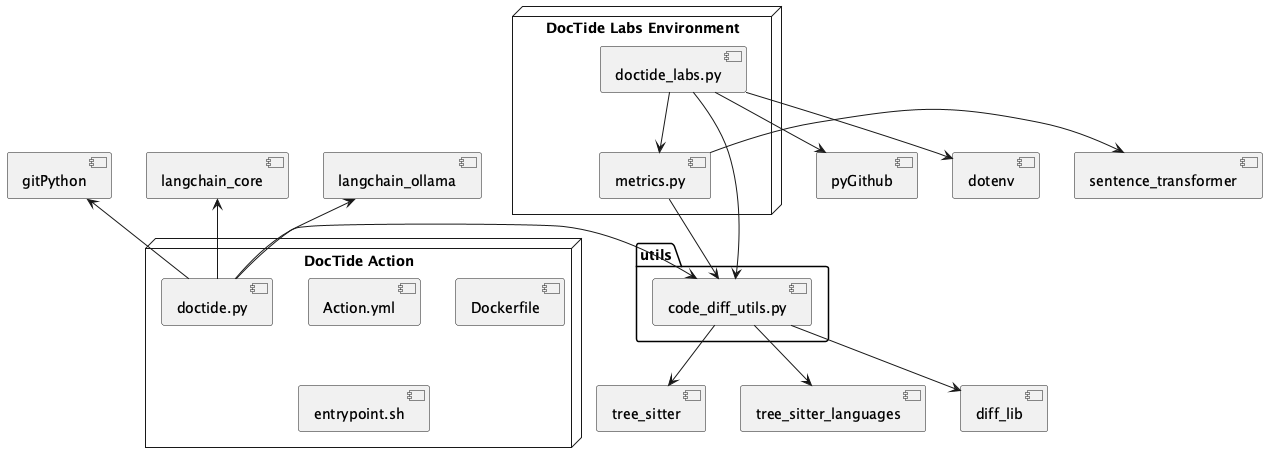
\includegraphics[width=0.7\linewidth]{Figures/component_diagram.png}
\caption{doctide.py dependencies and component structure}
\label{fig:components}
\end{figure}
\subsubsection*{gitPython}
GitPython\footnote{https://gitpython.readthedocs.io/en/stable/index.html} is used to have easy abstraction of git objects, enableing seamless interaction with a git repository. By passing the path to the working directory of the git repository of a system to the Repo("path") function, the system gets access to a pointer to the whole git repository. Which is easy in a GitHub Runner where the working directory is the equivalent to the working directory of the callers repository. It is now straight forward to create a branch and commit the generated function level documentations to that branch. And by creating a diff object between the most resent commit(HEAD) and second most resent commit (HEAD\(\sim \)1) using the Repo.head.commit and Commit.diff function, the most resent changes is identified which may call for generating and updating function-level documentation.
\subsubsection*{langchain}
Langchain is a framework for implement LLMs into a programming system. It is the core component in DocTide as it provides the local LLM which is used to generate the function-level documentation. DocTide uses the ollama service provided through \textbf{Langchain\_ollama.ChatOllama}\footnote{\url{https://python.langchain.com/api_reference/ollama/chat_models/langchain_ollama.chat_models.ChatOllama.html#langchain_ollama.chat_models.ChatOllama}}. Ollama is a vast library for LLMs which can be downloaded and run locally on a machine. Through the ChatOllama interface it is possible to specify which exact model from the Ollama library you wishes to use. To prompt the chosen model, the \textbf{langchain\_core.prompts.ChatPromptTemplate}\footnote{\url{https://python.langchain.com/api_reference/core/prompts/langchain_core.prompts.chat.ChatPromptTemplate.html#langchain_core.prompts.chat.ChatPromptTemplate}} offers a template to wrap the prompt for it to be in the right format for the ChatOllama.invoke function, which prompts the LLM with the given ChatPromptTmplate.
\subsubsection*{code\_diff\_utils.py}
Is a module created to seamlessly interact with the functionalities of tree-sitter (\ref{sec:tree-sitter}) and diff\_lib (\ref{sec:difflib}). Connecting tree-sitters ability to generate an abstract syntax tree (AST) for source code and diff\_libs ability to make diffs between two contexts, makes a reusable module for both doctide.py and doctide\_labs.py to avoid a lot of redundant code, and to have a framework which is easy to build new functionalities into, without having to build all the fundamentals again. This is done by the main function "extract\_data", which creates the AST of the source code, gain an understanding of which lines in the code has been modified and the traverses through the tree, and upon meeting a "function\_definition" node, it uses the handler function provided as an argument to do a specific task, which uses a helper function to identify a comment node. This ensures that the whole system follows the same logic on how the functions and function-level comments are identified, and is easy to modify and add functionalities by just making new handler functions.

\subsubsection*{tree-sitter}
\label{sec:tree-sitter}
To acquire contextual understanding of the modified files, an abstract syntax tree(AST) is created by passing the files with tree-sitter. An AST makes a tree like structure of the code, based on tokens which represents the building block of the code, so no matter what language the code was written in, the AST gives an abstract standardization of the code, which make it possible to processes files based on tokens instead of specific implementations. DocTide specifically uses the ASTs ability to identify function blocks and their associated comment style documentation. This also allows portability, in the future work of DocTide, since tree-sitter supports a large amount of programming languages, and can parse them into ASTs making it possible to analyze not only python but all the supported languages.

\subsubsection*{diff\_lib}
\label{sec:difflib}
Is a tool used to get the diff between the context of two versions of a file and therefor does not need a git reference to a commit to make a diff, which makes it quite flexible. To avoid a lot of redundant code between doctide.py and doctide\_labs.py in the analysis of the AST and which line were changed in the given two commits/contexts, the flexibility of diff\_lib was proven helpful as doctide.py and doctide\_labs.py uses two different tools to interact with git, gitPython and pyGitHub, which in terns also handles the way to look at diffs differently. But with diff\_lib, git is not relevant, and now both systems can use the code\_diff\_utils.py module

\subsection{Deployment as a GitHub Action}
To be able to integrate DocTide into a GitHub CI- pipeline, DocTide is deployed and accessible as a packaged Docker container action via the GitHub Marketplace, this section will go through how this is setup following the setup guide provided by GitHub \footnote{\url{https://docs.github.com/en/actions/sharing-automations/creating-actions/creating-a-docker-container-action}}. Public GitHub Actions are deployed to the GitHub Marketplace, wherefrom users are able to learn about the action and how to include it into there workflow. For DocTide to work as an action three files are necessary: Action.yml, Dockerfile and entrypoint.sh. 

\textbf{Action.yml} is a metadata file, which defines the setup for DocTide. It describes shortly what DocTide is and specifies its inputs and outputs and how it should be run. The latter is where it is specified that it uses docker to build an image of DocTide using the Dockerfile. 

The \textbf{Dockerfile} specifies the files DocTide consists of and where their source code is, such that it can be build into an image. 

Lastly the \textbf{entrypoint.sh} is the shell script which is run by the GitHub Runner (\Cref{sec:githubRunner}), this executes the login to GitHub via the Runners GitHub Token, installs the necessary python dependencies, installs Ollama and the chosen LLM, runs doctide.py and lastly commits generated function-level documentations to the callers branch. Which is what creates the pull request for the developers to modify or accept as is.
\subsubsection{Technical Design as an autonomous agent}
\textbf{Profiling}

DocTide has been given the specific role as a document assistance through the prompt given to the \textcolor{red}{LLM-model} as shown in \Cref{lst:prompt}

\begin{lstlisting}[language=Python, label={lst:prompt}, caption=Prompt used for the LLM]
    """
    You are a documentation assistant.

    ## Instructions:
    - Write a function-level documentation for the provided function, following best documentation practice for {program_language}
    Return **only** the comment

    ## Code:
    {code}
    """
\end{lstlisting}
\textbf{Memory}
\\
DocTide has a unified \textit{memory structure}, which means that information perceived from the environment only exist in local states inside the agent, and does not persist from run to run. The \textit{write operation} fetches the 'HEAD' commit and makes a diff with the 'HEAD\(\sim \)1'\footnote{The second latest commit on a repository} commit, identifying the latest changes to the repository. The \textit{memory format} of the diff is a structured list saved as diff\_files. The \textit{read operation} in DocTide is fairly simple as it just use the parameters \{program\_language\} and \{code\}, which is set by the planing module\ref{sec:planning module}, and read into the prompt.
\\ \\
\textbf{Planing and Action}
\label{sec:planning module}
The planing module is fairly simple, and does not rely on an LLM to plan the actions, but follows the sequence of the python script that is the backbone of the agent. \Cref{lst:plan_seq} shows as pseudo code the sequential order in which DocTide executes the actions following the the static plan. Given the simplistic nature DocTide as an autonomous agent, \ref{lst:plan_seq} also shows shows the entirety of the \textit{action space} for DocTide.

\begin{lstlisting}[language=Python, label={lst:plan_seq}, caption=The plan sequence of DocTides actions]
    - checkout_to_agent_branch
    for modified files:
        - detect_language
        - identify_modified_methods
            for modified methods:
            - generate_comment
            - validate_comment
    - commit_comments
    - write_to_testfile
\end{lstlisting}

\noindent
The \textit{production} of \textbf{write\_to\_testfile} is \textit{action via memory recollection}, as 
this action is triggered based on a 'testing' flag, read from the environment through memory. The remaining actions does all have \textit{action via plan following} as their production, meaning that they sequentially follow the plan. \textbf{detect\_language}, and \textbf{identify\_modified\_functions} has \textit{Environment Exploration} as their \textit{goal}, meaning the actions are aimed at deepening the agents understanding about its environment. The rest of the actions has \textit{Task Completion} as their \textit{goal}. The \textit{impact} of the actions is as followed:
\\\\
\textbf{checkout\_to\_agent\_branch:} is \textit{changing environment} of the agent, as the action serves to create a new branch for the agent to run on, and to checkout to this, effectively changing the state of the repository the agent is executing within.
\\ \\
\textbf{detect\_language:} extends the information know from the environment by detecting the language of the modified file, thus changing the \textit{internal state} of the agent.
\\ \\
\textbf{identify\_modified\_functions:} changes the \textit{internal state} of the agent by identifying which of the methods in the file has been modified in the latest commit.
\\ \\
\textbf{generate\_comment:} generates a method level comment for the modified method, adding this to the \textit{internal state} of the agent.
\\ \\
\textbf{validate\_comment:} handles validation of the generated method level comment, making sure that it follows the expected format and that it is not executable code. Based on the outcome of this validation, it then performs an \textit{action call} of the \textit{commit\_comments} action.
\\ \\
\textbf{commit\_comments:} handles add, commit and push of the newly generated method levels comments, thus \textit{changing the environment} of the agent.
\\ \\
\textbf{write\_to\_testfile:} if the agent is run with the 'testing' flag set to true, this action \textit{changes the environment} by handling writing test-data to a csv-file.

\subsection{Choice of LLM model}
The LLM which runs the code generation is the LLama 3.2 with 3 billion parameters. Its size is 2 gb which fits nicely to the hardware limits of the GitHub Runner (\Cref{sec:githubRunner})
